\documentclass[11pt,a4paper]{article}

\usepackage[utf8]{inputenc}
\usepackage{graphicx}
\usepackage{float}
\usepackage{titlesec}
\usepackage[singlespacing]{setspace}
\usepackage[left=2.5cm,right=2.5cm,top=2cm,bottom=2cm]{geometry}

\setlength{\parskip}{5pt plus 1 pt minus 1 pt}
\titlespacing\section{0pt}{3pt}{3pt}
\titlespacing\subsection{3pt}{3pt}{3pt}

\begin{document}

\begin{center}
{\Large Homework Sheet 05}
\end{center}

\thispagestyle{empty}
\pagestyle{empty}

\section*{1}

A 3-layered architectural style consists of 3 hierarchical layers,
while a 3-tier architecture consists of 3 tiers, which are not
necessariliy hierarchical. The layers are also seen more in a functional
way, while the tiers are objects interacting with each other.

\section*{2}

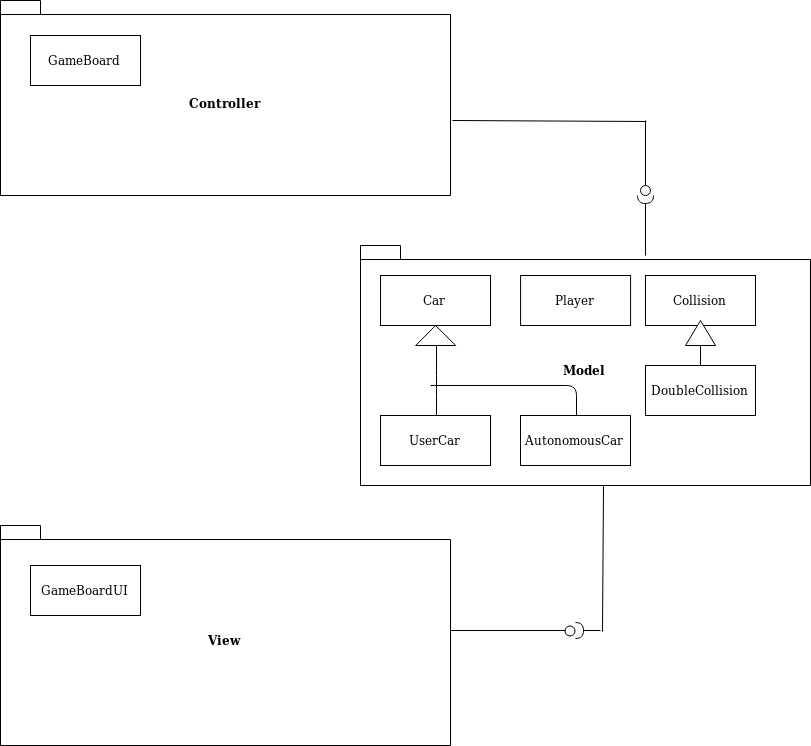
\includegraphics[width=15cm]{dg.png}

\end{document}
